\section{Lineare Abbildungen}

Lineare Abbildungen sind Abbildungen von einem Vektorraum in einen Vektorraum, die die lineare Struktur erhalten. Lineare Abbildungen nennt man in verschiedenen Teilgebieten der Mathematik auch lineare Transformationen, lineare Operatoren oder auch Homomorphismen von Vektorräumen.  

\subsection{Beispiele von linearen Abbildungen}
In diesem Abschnitt sei der zugrundeliegende Körper $ \K = \R $.

IM AUFBAU: Bilder - Quadrat mit einem Piktogramm drin. 

\subsubsection{90°-Drehung}
	90°-Drehung mit Drehzentrum in $ 0 $ im Gegenuhrzeigersinn.\\
	$ F: \R^2 \to \R^2, (x_1,x_2) \mapsto (-x_2,x_1) $
	
\subsubsection{Projektion in $ \R^3 $}
	$ F : \R^3 \to \R^3, (x_1,x_2,x_3) \mapsto (x_1, x_2, 0) $

\subsubsection{Projektion von $ \R^3 $  nach $ \R^2 $ }
	$ F : \R^3 \to \R^2, (x_1,x_2,x_3) \mapsto (x_1, x_2) $

\subsubsection{Punktspiegelung}
	Spiegelung an der $ 0 $.\\
	$ F : x = (x_1, x_2) \mapsto -x = (-x_1, -x_2) $
	
\subsubsection{Spiegelung an einer Geraden}
	Spiegelung an $ \R \times \{0\} $ ($ x_1 $-Achse).
	$ F: \R^2 \to \R^2, (x_1, x_2) \mapsto (x_1, -x_2) $

\subsubsection{Scherung}
	$ F: \R^2 \to \R^2, (x_1, x_2) \mapsto (x_1 + x_2, x_2) $

\subsubsection{Streckung}
	$ F: \R^2 \to \R^2, F: (x_1, x_2) \mapsto (x_1, 2 \cdot x_2) $

\subsubsection{Zyklische Verschiebung der Komponenten}
	Sei $ n \in \N $. $ F : \R^n \to \R^n, (x_1, \ldots, x_n) \mapsto (x_n, x_1, \ldots, x_{n-1}) $.\\[10pt]
	Die vorigen Abbildungen haben das Folgende gemeinsam: jede Komponente von $ F(x) $ ist Linearkombination der Komponenten von $ x $ mit konstanten Koeffizienten.

\subsection{Lineare Abbildungen für allgemeine Vektorräume}
\subsubsection{Lineare Abbildung}
Seien $ V $ und $ W $ Vektorräume über $ \K $. Sei $ F: V \to W $. Die Abbildung $ F $ heißt linear, falls:

\setlength{\myindent}{
	\maxof{
		\widthof{(L1)}
	}{
		\widthof{(L2)}
	}
}
\advance\myindent by \the\labelsep

\begin{itemize}
	\item [(L1)]
		$ F(v+w) = F(v) + F(w) \quad \forall v,w \in V $
	\item [(L2)]
		$ F(\lambda v) = \lambda F(v) \quad \forall v \in V, \forall \lambda \in \K $
\end{itemize}
\begin{bem}
	Offensichtlich gelten (L1) und (L2) genau dann, wenn folgendes gilt:
	\begin{itemize}[leftmargin=\myindent]
		\item[(L)]
			$ F(\lambda v + \mu w) = \lambda F(v) + \mu F(w) \quad \forall v,w \in V, \forall \lambda, \mu \in \K $
	\end{itemize}
\end{bem}

\subsubsection{Lineare Abbildungen und die Grundbegriffe für Vektorräume}
\begin{propn}
	Seien $ V $ und $ W $ Vektorräume über $ \K $. Sei $ F: V \to W $ linear. Dann gilt:
	\begin{enumerate}
		\item
			$ F(0) = 0 $ und $ F(v-w) = F(v) - F(w) \quad \forall v,w \in V $
		\item
			$ F(\lambda_1 v_1 + \ldots + \lambda_n v_n) = \lambda_1 F(v_1) + \ldots + \lambda_n F(v_n) $ \\ $ \forall n \in \N_0, \lambda_1, \ldots, \lambda_n \in \K, v_1, \ldots, v_n \in \K $
		\item
			Ist $ (v_i)_{i \in I} $ eine linear abhängige Familie von Vektoren aus $ V $, dann ist $ (F(v_i))_{i \in I} $ eine linear abhängige Familie von Vektoren aus $ W $.
		\item
			Ist $ V' $ Untervektorraum von V, dann ist $ F(V') $ Untervektorraum von $ W $.
		\item
			Ist $ W' $ Untervektorraum von W, dann ist $ F^{-1}(W') $ Untervektorraum von $ V $.
		\item
			$ \dim(F(V)) \leq \dim(V) $
		\item
			Ist $ F $ bijektiv, dann ist auch $ F^{-1} : W \to V $ linear.
	\end{enumerate}
\end{propn}
\begin{proof}
	\begin{enumerate}
		\item
			$ F(x) = F(0+x) = F(0) + F(x) \quad \forall x \in V $
			$ \Rightarrow F(0) = F(x) - F(x) = 0 $
		\item
			folgt durch das iterative Anwenden von (L1) und (L2):
			\begin{align*}
				 F(\lambda_1 v_1 + \cdots + \lambda_n v_n ) &= F(\lambda_1 v_1 + \cdots + \lambda_{n-1} v_{n-1} ) + F(\lambda_n v_n) \\
				 &= F(\lambda_1 v_1 + \cdots + \lambda_{n-1} v_{n-1} ) + \lambda_n F(v_n)
			\end{align*}
			und so weiter für alle $ n \in \N $.
		\item
			Wenn $ (v_i)_{i \in I} $ linear abhängig ist, dann existieren $ \lambda_{i_1}, \ldots, \lambda_{i_n} \in \K $ (nicht alle Null) und $ v_{i_1}, \ldots, v_{i_n} $ mit $ i_1, \ldots, i_n \in I $ ($ n \in \N $), sodass $ \lambda_{i_1} v_{i_1} + \cdots + \lambda_{i_n} v_{i_n} = 0 $. Das Anwenden von $ F $ mit der Berücksichtigung von (i) und (ii) ergibt
			\begin{equation*}
				0 = F(0) = F(\lambda_{i1} v_{i1} + \cdots + \lambda_{in} v_{in} ) = \lambda_{i1} F(v_{i1}) + \cdots + \lambda_{in} F(v_{in}).
			\end{equation*}
			Das zeigt die lineare Abhängigkeit von $ (F(v_i))_{i \in I} $.
		\item
			$ F(V') \neq \emptyset $, denn $ 0 \in V' $ und somit $ 0 = F(0) \in F(V') $. Wenn $ w_1, w_2 \in F(V') $, dann gilt $ w_1 = F(v_1), w_2 = F(v_2) $ für gewisse $ v_1, v_2 \in V' $. $ V' $ ist Untervektorraum von $ V $ und somit $ v_1 + v_2 \in V' \Rightarrow w_1 + w_2 = F(v_1) + F(v_2) = F(v_1 + v_2) \in F(V') $.
			
			Analog zeigt man auch, dass für jedes $ \lambda \in \K $ und jedes $ w \in F(V') $ die Bedingung $ \lambda w \in F(V') $ gilt.
		\item
			$ F^{-1}(W') \neq \emptyset $, denn $ 0 \in F^{-1}(W') $ (d.h. $ 0 = F(0) \in W' $).
			
			Seien $ v_1, v_2 \in F^{-1}(W') $, d.h. $ F(v_1), F(v_2) \in  W' $. Es folgt $ F(v_1 + v_2) = F(v_1) + F(v_2) \in W' $. D.h. $ v_1 + v_2 \in F^{-1}(W') $.
			
			Analog zeigt man, dass $ \lambda v \in F^{-1}(W') $ für alle $ \lambda \in \K $ und alle $ v \in F^{-1}(W') $ gilt.
		\item
			Übung.
		\item
			Übung. \qedhere
	\end{enumerate}
\end{proof}

\subsubsection{Komposition von linearen Abbildungen}

\begin{propn}
	Seien $ U, V $ und $ W $ Vektorräume über $ \K $. Seien $ G : U \to V $ und $ F : V \to W $ linear. Dann ist auch $ F \circ G $ linear.
\end{propn}
\begin{proof}
	Seien $ u_1, u_2 \in U $. Dann ist wegen der Linearität von $ G $ und $ F $
	\begin{align*}
		(F \circ G)(u_1+u_2) &= F(G(u_1+u_2)) \\
		&= F(G(u_1)+G(u_2)) \\
		&= F(G(u_1))+F(G(u_2)) \\
		&= (F \circ G)(u_1) + (F \circ G)(u_2).
	\end{align*}
	Analog verifiziert man, dass $ (F \circ G)(\lambda u) = \lambda (F \circ G)(u) $ für alle $ \lambda \in \K, u \in U $ gilt.
\end{proof}

\subsubsection{Vektorräume der linearen Abbildungen}

Seien $ V$ und $ W $ Vektorräume über $ \K $. Wir bezeichnen durch $ \Lin_\K(V,W) $ die Menge aller linearen Abbildungen von $ V $ nach $ W $.

\begin{propn}
	Seien $ V $ und $ W $ Vektorräume über $ \K $. Die Menge $ \Lin(V,W) $ mit den Operationen $ (F+G)(v) := F(v) + G(v) \quad \forall v \in V $ (Addition) und $ (\lambda \cdot F)(v) := \lambda \cdot F(v) \quad \forall \lambda \in \K, v \in V $ (Skalarmultiplikation) ist ein Vektorraum.
\end{propn}
\begin{proof}
	Wir bemerken, dass die Menge $ W^V $ mit der Addition und Skalarmultiplikation wie oben ein Vektorraum ist (der Beweis ist direkt). Weil $ \Lin(V,W) \subseteq W^V $ gilt, reicht es zu zeigen, dass $ \Lin(V,W) $ ein Untervektorraum von $ W^V $ ist.
	
	Die \emph{Nullabbildung} von $ V $ nach $ W $ (d.h. $ F $ mit $ F(v) = 0 $ für jedes $ v \in V $) gehört zu $ \Lin(V,W) $. Daher ist $ \Lin(V,W) \neq \emptyset $.
	
	Seien $ F_1, F_2 \in \Lin(V,W) $. Zu zeigen: $ F_1 + F_2 \in \Lin(V,W) $. Seien $ v_1, v_2 \in V $. Dann ist
	\begin{align*}
		(F_1+F_2)(v_1+v_2) &= F_1(v_1+v_2) + F_2(v_1+v_2)\\
		&= F_1(v_1) + F_1(v_2) + F_2(v_1) + F_2(v_2)\\
		&= (F_1(v_1)+F_2(v_1)) + (F_1(v_2)+F_2(v_2))\\
		&= (F_1+F_2)(v_1) + (F_1+F_2)(v_2).
	\end{align*}
	
	Analog zeigt man, dass $ (F_1+F_2)(\lambda v) = \lambda(F_1+F_2)(v) \quad \forall\lambda\in\K, v \in V $ gilt, und dass für $ \mu \in \K $ und $ F \in \Lin(V,W) $ die Bedingung $ \mu F \in \Lin(V,W) $ erfüllt ist.
\end{proof}

\subsubsection{Lineare Abbildungen eines Vektorraums}

Sei $ V $ Vektorraum über $ \K $. Wir führen die Bezeichnung $ \Lin_\K(V) := \Lin_\K(V,V) $ ein. Wir nennen die Elemente von $ \Lin_\K(V) $ die linearen Abbildungen des Vektorraums $ V $.

%\begin{quotation}
%	\noindent Die Algebraika nennen lineare Abbildungen Holomorphismen und lineare Abbildungen eines Vektorraums Endomorphismen. Ich sehe keinen Grund, diese Begriffe einzuführen. Ich mag lineare Abbildung.\\[10pt]
%	Vielleicht sollte man ein Wörterbuch erstellen:
%	\begin{itemize}
%		\item
%			Algebra: Holomorphismus, \\
%			Klartext: lineare Abbildung
%		\item
%			Algebra: Endomorphismus, \\
%			Klartext: lineare Abbildung in einem Vektorraum
%	\end{itemize}
%\end{quotation}

\begin{propn}
	Sei $ V $ Vektorraum über $ \K $. Dann ist die Menge $ \Lin(V) $ mit den Operationen $ (F+G)(v) := F(v)+G(v) \quad \forall v \in V, \forall F,G \in \Lin(V) $ (Addition) und $ (F \cdot G)(v) := (F \circ G)(v) \quad \forall v \in V, \forall F,G \in \Lin(V) $ (Multiplikation) ein Ring mit Eins.
\end{propn}
\begin{proof}
	Da $ (V,+) $ eine kommutative Gruppe ist, ist auch $ (\Lin(V),+) $ eine kommutative Gruppe. Die Multiplikation ist assoziativ, weil $ \circ $ (Komposition) assoziativ ist. Die beiden Distributivgesetze gelten (der Beweis ist direkt). Das neutrale Element ist $ \id_V $ (identische Abbildung auf $ V $).
\end{proof}

\clearpage
\subsection{Matrizenmultiplikation und lineare Abbildungen für Räume $ \K^n $}

Eine lineare Abbildung von $\K^n$ nach $\K^m$ kann durch eine $m \times n$ Matrix beschrieben werden. Die Komposition von zwei linearen Abbildungen $F$ und $G$ mit $\K^n \xrightarrow{G} \K^p \xrightarrow{F} \K^m$ entspricht dann dem Produkt von zwei Matrizen. 

\subsubsection{Multiplikation von Matrizen}

Seien $ A = {{(a_{ij})}_{i=1}^m}_{j=1}^n \in \K^{m \times n} $ und $ B = {{(b_{jk})}_{j=1}^n}_{k=1}^p \in \K^{n \times p} $ ($ m,n,p \in \N $). Dann heißt $ C = {{(c_{ik})}_{i=1}^m}_{k=1}^p := A \cdot B \in \K^{m \times p} $ mit 
\[
	 c_{ik} := \sum_{j=1}^{n} a_{ij}b_{jk} 
\] das Produkt von $ A $ und $ B $. Das heißt, $c_{ik}$ hängt von der $i$-ten Zeile von $A$ und der $k$-ten Spalte von $B$ ab: 
\begin{equation*}
	\begin{pmatrix}
		\phantom{a} && \phantom{a} \\
		 a_{i1} & \ldots & a_{in} \\
		\phantom{a} && \phantom{a}
	\end{pmatrix}
	\cdot
	\begin{pmatrix}
		\phantom{b} & b_{1k} & \phantom{b} \\
		& \vdots & \\
		& b_{nk} &
	\end{pmatrix}
	=
	\begin{pmatrix}
		\phantom{c} && \phantom{c} \\
		& c_{ik} & \\
		\phantom{c} && \phantom{c}
	\end{pmatrix}
\end{equation*}

\begin{bsp}[$ 2\times2 $ Matrizen]\
	\begin{align*}
		\begin{pmatrix}
			a_{11} & a_{12} \\
			a_{21} & a_{22}
		\end{pmatrix}
		\begin{pmatrix}
			b_{11} & b_{12} \\
			b_{21} & b_{22}
		\end{pmatrix}
		&=
		\begin{pmatrix}
			c_{11} & c_{12} \\
			c_{21} & c_{22}
		\end{pmatrix} 
	\end{align*}
	\begin{align*}
		c_{11} &= a_{11}b_{11} + a_{12}b_{21}  & 
c_{12} &= a_{11}b_{12} + a_{12}b_{22} \\
c_{21} &= a_{21}b_{11} + a_{22}b_{21}  &
c_{22} &= a_{21}b_{12} + a_{22}b_{22}
	\end{align*}
\end{bsp}

\begin{bem}
	Die Matrix-Vektor-Multiplikation ist ein Spezialfall der Matrix-Matrix-Multiplikation. Für
	 $ A = (a_{ij}) \in \K^{m \times n} $ und $ x = (x_1, \ldots, x_n) \in \K^n $ Dann ist $Ax $ ein Element von $\K^m$ mit 
	\begin{equation*}
		Ax =
		\begin{pmatrix}
			a_{11} & \cdots & a_{1n} \\
			 &  \vdots &  \\
			a_{m1} & \cdots & a_{mn}
		\end{pmatrix}
		\begin{pmatrix}
			x_1 \\
			\vdots \\
			x_n
		\end{pmatrix}
		=
		\begin{pmatrix}
			a_{11}x_1 + \ldots + a_{1n}x_n \\
			\vdots \\
			a_{m1}x_1 + \ldots + a_{mn}x_n
		\end{pmatrix}
	\end{equation*}
	wobei man hier die Elemente aus $\K^n$ und $\K^m$ als Spalten interpretiert. 
	
	Nun kann auch ein LGS mit $m$ Gleichungen und $n$ Unbekannten kompakt als $A x = b$ beschrieben werden. 
\end{bem}

\begin{bem}
	Wenn wir im Produkt $A B$ die Matrix $B$ spaltenweise als 
	\[
		B = \begin{pmatrix} 
			| & & | 
			\\ b_1 & \cdots & b_p
			\\ | & & | 
		\end{pmatrix} 
	\]
	so kann auch das Produkt $AB$ spaltenweise als 
	\[
		AB =
		\begin{pmatrix} 
		| & & | 
		\\ A b_1 & \cdots & A b_p
		\\ | & & | 
		\end{pmatrix}
	\]
	dargestellt werden. Das heißt: die Matrix $A$ (er erste Faktor) wirkt auf jede Spalte der  Matrix $B$ (der zweite Faktor)
\end{bem}

\begin{bem}
	Durch ein Matrix-Vektor-Produkt $A x$ mit $A \in \K^{m \times n}$ und $x \in \K^n$ können Linearkombinationen von Vektoren aus $\K^m$ beschrieben werden, indem man die Matrix $A$ spaltenweise interpretiert. Ist 
	\[
		A = \begin{pmatrix} 
			| & & |
	\\		a_1 & \cdots & a_n 
	\\	| & & |
		\end{pmatrix} 
	\]
	und $x=(x_1,\ldots,x_n) \in \K^n$ so gilt 
	\[ 
		Ax = x_1a_1 + \ldots + x_na_n.
	\]
	Das heißt, $A x$ ist die Linearkombination der Spalten von $A$, deren Koeffizienten die Komponenten des Vektors $x$ sind. 
\end{bem}

\begin{bem}
	Nützliche Links: {\\ \scriptsize 
	 \url{https://de.wikipedia.org/wiki/Matrizenmultiplikation} \\ 
	 \url{https://en.wikipedia.org/wiki/Matrix_multiplication} } 
\end{bem} 

\begin{bem}[Matrizenmutliplikation in den Wirtschaftlichenkontexten] 
	Man betrachte: 
	\begin{itemize} 
		\item Nutrienten (Kohlenhydrate, Fette, Proteine, Vitamine, Mineralstoffe, Wasser)
		\item Ingredienten (Zucker, Mehl, Eier, Tomaten usw.). 
		\item Gerichte (Kartoffelsalat, Eierschecke usw.). 
	\end{itemize} 
	
	$A = (a_{g,i})_{g,i}$ - Gericht-Ingredienten-Matrix : wie viele Einheiten des Ingredienten pro ein Gericht (eine Einheit des Gerichts). 
	
	$B = (b_{i,n})_{i,n}$  - Ingredienten-Nutrienten-Matrix: wie viele Einheiten des Nutrienten pro eine Einheit des Ingredienten. 
	
	$C = A B$ ist die -Gericht-Nutrienten-Matrix: wie viele Einheiten des Nutrienten pro ein Gericht (eine Einheit des Gerichts). 
	\[
		c_{g,n} = \sum_{i} a_{g,i} b_{i,n}.
	\]
	
	Ähnliche Art Kalkulatinen, die man als Multiplikation von Matrizen auffassen kann, sind omnipräsent in den wirtschaftlichen Kontexten. 
\end{bem} 

\subsubsection{Matrix einer linearen Abbildung von $ \K^n $ nach $ \K^m $}


\begin{propn}
	Sei $ F : \K^n\to \K^m $ linear ($ m,n \in \N $). Dann existiert eine eindeutige Matrix $ A \in \K^{m \times n} $ mit $ F(x) = Ax $ für alle $ x \in \K^n $. Es gilt \[
		 A = \begin{pmatrix} 
		 | & & |
		 \\ F(e_1) & \cdots &  F(e_n) 
		 \\ | & & | \end{pmatrix}, 
	\]
	d.h., die Spalten von $A$ entstehen durch die Auswertung von $F$ auf den Vektoren der Standardbasis $e_1,\ldots,e_n$. 
\end{propn}
\begin{proof}
	Sei $ x = (x_1, \ldots, x_n) \in \K^n $. Dann ist $ x = x_1e_1 + \ldots + x_ne_n $. Somit gilt
	\begin{equation*}
		F(x) = F(x_1e_1 + \ldots x_ne_n) = x_1F(e_1) + \ldots + x_nF(e_n) = 
		\begin{pmatrix} 
		| & & |
		\\ F(e_1) & \cdots &  F(e_n) 
		\\ | & & | \end{pmatrix} 
		\begin{pmatrix}
		x_1 \\ \vdots \\ x_n
		\end{pmatrix}.
	\end{equation*}
	Es bleibt die Eindeutigkeit von $ A $ zu zeigen. Sei $ F(x) = Ax $ für alle $ x \in \K^n $. Für $ x = e_i $ ($ i \in \{ 1, \ldots, n \} $) gilt $ F(e_i) = Ae_i $. Dabei ist $ Ae_i $ die $ i $-te Spalte von $A$. Das zeigt die Eindeutigkeit. 
\end{proof}

\noindent Für $ F $ und $ A $ wie in der vorigen Proposition nennen wir $ A $ die Matrix von $ F $. $ F $ heißt die \emph{durch $ A $ definierte lineare Abbildung.}

\begin{bsp} 
 Die Drehung $F : \R^2 \to \R^2$ um $135^\circ = 90^\circ + 45^\circ$ im Gegenuhrzeigersinn wird durch die Drehung der Standarbasisvektoren $e_1$ und $e_2$ berechnet. $F(x) = x_1 F(e_1) + x_2 F(e_2)$. Das bedeutet salopp gesagt, Folgendes. Um $x = \begin{pmatrix} x_1 \\ x_2 \end{pmatrix}$ zu drehen, müssen $e_1$ und $e_2$ gedreht werden; dann dreht sich $x$ mit. Stellen Sie sich vor, $x$ ist einen Karton eingepackt, dessen Platzierung durch $e_1$ und $e_2$ bestimmt wird. Nun wird der Karton gedreht, indem man $e_1$ und $e_2$ dreht, sodass sich $x$ dadurch mitdreht. Für $F(e_1)$ und $F(e_2)$ hat man aus den geometrischen Betrachtungen die Darstellung 
 \begin{align*} 
 		F(e_1)  & = {\color{green!50!black} \begin{pmatrix}  -\frac{1}{\sqrt{2}} \\ \frac{1}{\sqrt{2}} 
 		\end{pmatrix} }
 	& 
 		F(e_2)  & = {\color{red!80!black} \begin{pmatrix}  -\frac{1}{\sqrt{2}} \\ -\frac{1}{\sqrt{2}}. 
\end{pmatrix} } 
 \end{align*} 
Das zeigt, 
\[
	F(x)  = x_1 \begin{pmatrix}  -\frac{1}{\sqrt{2}} \\ \frac{1}{\sqrt{2}} 
	\end{pmatrix}  + x_2 \begin{pmatrix}  -\frac{1}{\sqrt{2}} \\ - \frac{1}{\sqrt{2}}. 
\end{pmatrix},
\]
oder in der Matrixform: 
\[
	F (x) = \begin{pmatrix} {\color{green!50!black} -\frac{1}{\sqrt{2}}} & { \color{red!80!black} -\frac{1}{\sqrt{2}}} \\
		{\color{green!50!black} \frac{1}{\sqrt{2}} } & { \color{red!80!black} - \frac{1}{\sqrt{2}}} \end{pmatrix} \begin{pmatrix} x_1 \\ x_2 \end{pmatrix}. 
\]
\begin{center} 
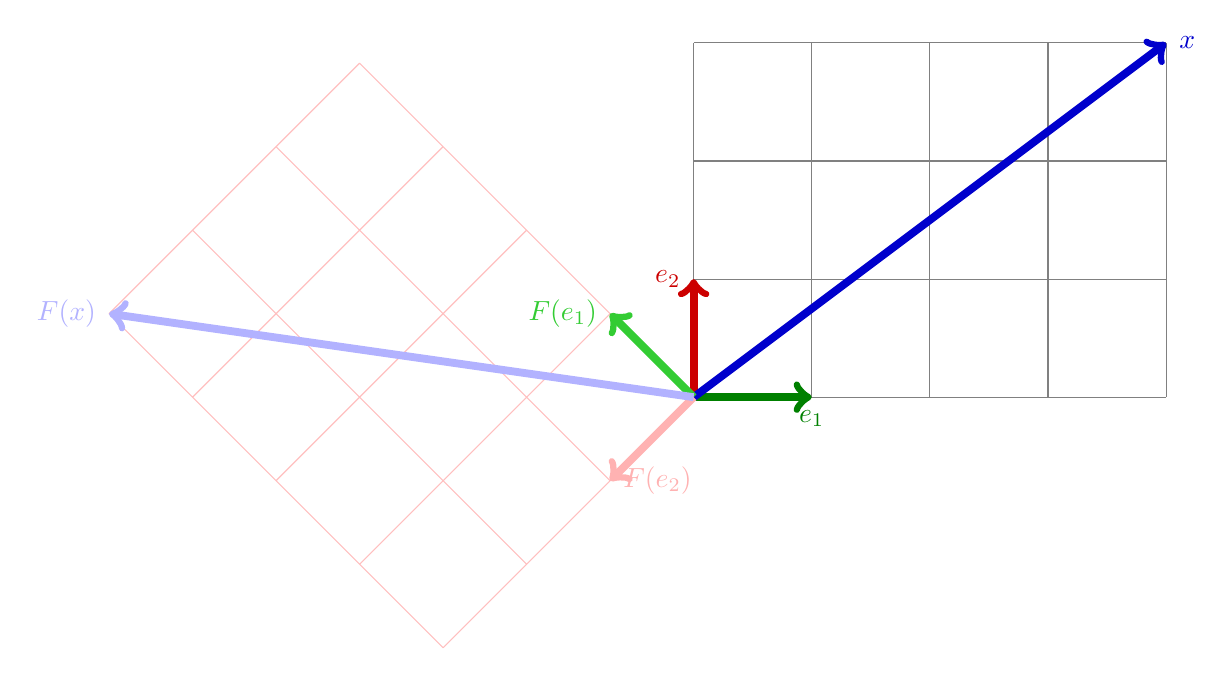
\begin{tikzpicture}[scale=1.5]
	\draw[gray] (0,0) grid (4,3);
	\draw[->,line width = 1mm,green!50!black] (0,0) -- (1,0) node[below]{$e_1$};
	\draw[->,line width = 1mm,red!80!black] (0,0) -- (0,1) node[left]{$e_2$};
	\draw[->,line width = 1mm,blue!80!black] (0,0) -- (4,3) node[right]{$x$};

	\draw[pink, rotate around={135:(0,0)}] (0,0) grid (4,3);
	\draw[->,line width = 1mm,green!60!gray, rotate around={135:(0,0)}] (0,0) -- (1,0) node[left]{$F(e_1)$};
	\draw[->,line width = 1mm,red!30!white, rotate around={135:(0,0)}] (0,0) -- (0,1) node[right]{$F(e_2)$} ;
	\draw[->,line width = 1mm,blue!30!white, rotate around={135:(0,0)}] (0,0) -- (4,3) node[left]{$F(x)$} ;
\end{tikzpicture} 
\end{center} 
\end{bsp} 

\begin{bsp}\
	\begin{itemize}
		\item  Identische Abbildung: $ F : \K^3 \to \K^3 $ mit $ F(x) = x $ für alle $ x \in \K^3 $.
		\begin{equation*}
			\begin{pmatrix} x_1 \\ x_2 \\ x_3 \end{pmatrix}  \mapsto \begin{pmatrix} 1 & 0 & 0 \\ 0 & 1 & 0 \\ 0 & 0 & 1 \end{pmatrix} \begin{pmatrix} x_1 \\ x_2 \\ x_3 \end{pmatrix}
		\end{equation*}
		\item Drehung um 90 Grad. $ \K = \R, (x_1,x_2) \mapsto (-x_2,x_1) $
		\begin{equation*}
			\left( \begin{matrix}
			x_1 \\ 
			x_2
			\end{matrix} \right)
			\mapsto
			\left( \begin{matrix}
			0 & -1 \\ 
			1 & 0
			\end{matrix} \right)
			\left( \begin{matrix}
			x_1 \\ 
			x_2
			\end{matrix} \right)
		\end{equation*}
		\item Projektion auf die Ebene $\R^2 \times \{0\}$ innerhalb von $\R^3$. $ (x_1,x_2,x_3) \mapsto (x_1,x_2,0) $
		\begin{equation*}
			\left( \begin{matrix}
			x_1 \\ 
			x_2 \\
			x_3
			\end{matrix} \right)
			\mapsto
			\left( \begin{matrix}
			1 & 0 & 0 \\ 
			0 & 1 & 0 \\
			0 & 0 & 0
			\end{matrix} \right)
			\left( \begin{matrix}
			x_1 \\ 
			x_2 \\
			x_3
			\end{matrix} \right)
		\end{equation*}
		\item Projektion auf die ersten beiden Koordinaten als Abbildung von $\R^3$ nach $\R^2$. $ (x_1,x_2,x_3) \mapsto (x_1,x_2) $
			\begin{equation*}
				\left( \begin{matrix}
				x_1 \\ 
				x_2 \\
				x_3
				\end{matrix} \right)
				\mapsto
				\left( \begin{matrix}
				1 & 0 & 0 \\ 
				0 & 1 & 0
				\end{matrix} \right)
				\left( \begin{matrix}
				x_1 \\ 
				x_2 \\
				x_3
				\end{matrix} \right)
			\end{equation*}
	\end{itemize}
\end{bsp}

\subsubsection{Matrix der Komposition von linearen Abbildungen}

\begin{thm}
	Seien $ l,m,n \in \N $, seien $ G:\K^n\to\K^m $ und $ F:\K^m\to\K^l $ linear. Sei $ B \in \K^{m \times n} $ die Matrix von $ G $ und sei $ A \in \K^{l \times m} $ die Matrix von $ F $. Dann ist $ AB $ die Matrix von $ F \circ G $.
\end{thm}
\begin{proof}
	Nach den Voraussetzungen gilt $ F(y) = Ay $ und $ G(x) = Bx $ für alle $ x \in \K^n $ und alle $ y \in \K^m $, oder als Diagramm:  	
	\begin{equation*}
		\K^l    \xleftarrow[A \in \K^{l \times m}]{\hspace{3ex} F(y) = B y \hspace{3ex}}   \K^m  \xleftarrow[B \in \K^{m \times n}]{\hspace{3ex}  G(x) = Ax \hspace{3ex}} \K^n
	\end{equation*} 

	
Daher gilt $ (F \circ G)(x) = F(G(x)) = F(Bx) = A \cdot (B \cdot x) $.
	
	Zu zeigen: $ A \cdot (B \cdot x) = (A \cdot B) \cdot x $. Sei $ x=(x_1,\ldots,x_n) $, sei $ A = {{(a_{ij})}_{i=1}^l}_{j=1}^m $ und sei $ B = {{(b_{jk})}_{j=1}^m}_{k=1}^n $. Man hat: 
	\begin{align*}
		\text{Die $ i $-te Komponente von $ A \cdot (B \cdot x) $ ist} & & &   \sum\limits_{j=1}^{m}a_{ij}\underbrace{\left( \sum\limits_{k=1}^{n}b_{jk}x_k \right)}_{\text{$ j $-te Komponente von $ Bx $}}, \vspace{3ex}
		\\ 		\text{Die $ i $-te Komponente von $ (A \cdot B) \cdot x $ ist} & & & \sum\limits_{k=1}^{n} \underbrace{\left( \sum\limits_{j=1}^{m}a_{ij}b_{jk} \right)}_{\substack{\text{die Komponente}\\ \text{ in der Position $ (i,k) $ von $ AB $}}} x_k
	\end{align*}
 	Durch das Auflösen der Klammern sieht man, dass diese beiden geschachtelten Summen mit der Summe
	\begin{equation}
		\sum\limits_{\substack{j \in \{1,\ldots,m\} \\ k \in \{1,\ldots,n\}}} a_{ij}b_{jk}x_k
	\end{equation}
	übereinstimmen. Das ergibt die Behauptung.
\end{proof}

%\begin{bsp}
%	$ \K = \R $
%	\begin{itemize}
%		\item
%			$ F : \R^2 \to \R^2 $
%
%			\begin{tikzpicture}
    \draw (0,0) -- (1,0) -- (1,1) -- (0,1) -- cycle;
    \node () at (0,0) [below left] {$ 0 $};
    \node () at (1,0) [below right] {$ l_1 $};
    \node () at (0,1) [above left] {$ l_2 $};
    
    \node () at (2,0.5) {$ \longmapsto $};
    
    \draw (3,0) -- (4,0) -- (4.5,1) -- (3.5,1) -- cycle;
\end{tikzpicture}
%		\item
%			$ G : \R^2 \to \R^2 $
%		
%			\begin{tikzpicture}
    \draw (0,0) -- (1,0) -- (1,1) -- (0,1) -- cycle;
    \node () at (2,0.5) {$ \longmapsto $};
\end{tikzpicture}
%	\end{itemize}
%\end{bsp}

\subsubsection{Rechenregeln für Matrizen}

Für $ m,n\in\N $ ist die Menge $ \K^{m \times n} $ aller Matrizen der Größe $ m \times n $ einen Vektorraum der Form $ \K^X $ mit $ X = \{ 1,\ldots,m \}\times\{ 1,\ldots,n \} $. Diese Vektorräume wurden in 3.1.1 eingeführt. Somit hat man für $ \K^{m \times n} $ Addition und Skalarmultiplikation. Etwa:
\begin{align}
	\left( \begin{matrix}
	a_{11} & a_{12} \\ 
	a_{21} & a_{22}
	\end{matrix} \right)
	+
	\left( \begin{matrix}
	a'_{11} & a'_{12} \\ 
	a'_{21} & a'_{22}
	\end{matrix} \right)
	&=
	\left( \begin{matrix}
	a_{11}+a'_{11} & a_{12}+a'_{12} \\ 
	a_{21}+a'_{21} & a_{22}+a'_{22}
	\end{matrix} \right)\\
	\lambda
	\left( \begin{matrix}
	a_{11} & a_{12} \\ 
	a_{21} & a_{22}
	\end{matrix} \right)
	&=
	\left( \begin{matrix}
	\lambda a_{11} & \lambda a_{12} \\ 
	\lambda a_{21} & \lambda a_{22}
	\end{matrix} \right)
\end{align}

\begin{thm}
	 Seien $ A,A'\in\K^{m \times n} $, $ B,B'\in\K^{n \times k}, C \in \K^{k \times p} $ ($n,k,p \in \N$) und $ \lambda\in\K $. Dann gilt:
	\begin{enumerate}[label=\normalfont(\roman*)]
		\item $ A \cdot ( B + B') = A \cdot B + A \cdot B' $
		\item $ (A + A') \cdot B = A \cdot B + A' \cdot B $
		\item $ A \cdot (\lambda B) = (\lambda A) \cdot B = \lambda (A \cdot B) $
		\item $ (A \cdot B) \cdot C = A \cdot (B \cdot C) $
		\item $ (A \cdot B)^\top = B^\top \cdot A^\top $
	\end{enumerate}
\end{thm}
\begin{proof}
	Die ersten drei Formeln sind einfach. Die letzten beiden Formeln sind Übungsaufgaben.
\end{proof}

\subsubsection{Die Einheitsmatrix}

Seien $ i,j\in\N $. Dann heißt
\begin{equation}
	\delta_{ij} =
	\begin{cases}
		1 & \text{falls $ i = j $}\\
		0 & \text{falls $ i \neq j $}
	\end{cases}
\end{equation}
das \emph{Kronecker Delta} von $ (i,j) $.

Für $ n\in\N $ heißt die Matrix $ I_n := (\delta_{ij})_{i,j=1}^n $ die Einheitsmatrix der Größe $ n \times n $. Wenn die Wahl von $ n $ klar ist, schreibt man auch $ I $. Oder auch: $ \I $. Etwa:
\begin{equation}
	I_3 =
	\left( \begin{matrix}
	1 & 0 & 0 \\ 
	0 & 1 & 0 \\ 
	0 & 0 & 1
	\end{matrix}  \right)
\end{equation}
Für jede Matrix $ A\in\K^{m \times n} $ ($ m,n\in\N $) gilt offensichtlich $ I_mA = AI_n = A $. Die durch $ I_n $ definierte Abbildung ist die identische Abbildung auf $ \K^n $.

\begin{propn}
	Sei $ n\in\N $. Dann ist $ \K^{n \times n} $ mit der Addition und Multiplikation von Matrizen ein Ring mit Eins.
	
	Das neutrale Element bzgl. der Multiplikation ist die Einheitsmatrix $ I_n $. Die Matrix in $ \K^{n \times n} $ ($ n\in\N $), deren Einträge alle gleich Null sind, wird die \emph{Nullmatrix} genannt und durch $ O $ bezeichnet.
\end{propn}
\begin{proof}
	Alle Ringeigenschaften lassen sich direkt verifizieren. Es sei bemerkt, dass man im Wesentlichen keinen Unterschied zwischen $ \K^{n \times n} $ und $ \Lin(\K^n) $ hat. Man sagt: die Ringe $ \K^{n \times n} $ und $ \Lin(\K^n) $ sind isomorph (die genaue Definition wird erstmal nicht angegeben; $ \rightsquigarrow $ gleich, aber nicht dasselbe).
\end{proof}

\subsubsection{Invertierbarkeit von Matrizen}

Sei $ n\in\N $ und $ A\in\K^{n \times n} $. Dann heißt $ A $ \emph{invertierbar}, falls eine Matrix $ B\in\K^{n \times n}$ mit $ BA = AB = I $ existiert. Für eine invertierbare Matrix $ A $ ist die Matrix $ B $ wie oben eindeutig bestimmt (Übungsaufgabe). Diese Matrix wird die \emph{inverse Matrix} von $ A $ genannt und durch $ A^{-1} $ bezeichnet.

\begin{propn}
	Sei $ n\in\N $, sei $ F:\K^n\to\K^n $ linear und sei $ A $ die Matrix von $ F $. Dann sind die folgenden Bedingungen äquivalent:
	\begin{enumerate}
		\item $ F $ ist invertierbar.
		\item $ A $ ist invertierbar.
	\end{enumerate}
	Wenn {\normalfont(i)} und {\normalfont(ii)} gelten, dann ist $ A^{-1} $ die Matrix der Abbildung $ F^{-1} $.
\end{propn}
\begin{proof}
	Direkte Folgerung von 4.3.2 und 4.3.3.
\end{proof}

\subsubsection{Eigenschaften der inversen Matrizen}

\begin{propn}
	Sei $ n\in\N $, seien $ A,B\in\K^{n \times n} $ invertierbare Matrizen. Dann sind $ A^{-1}, A^\top $ und $ AB $ invertierbar und es gilt:
	\begin{align}
		(A^{-1})^{-1} &= A\\
		(A^\top)^{-1} &= (A^{-1})^\top\\
		(AB)^{-1} &= B^{-1}A^{-1}
	\end{align}
\end{propn}
\begin{proof}
	Übungsaufgabe.
\end{proof}

\subsubsection{Allgemeine lineare Gruppe}

Für $ n\in\N $ ist die allgemeine lineare Gruppe als 
\begin{equation}
	\GL_n(\K) := \{ A\in\K^{n \times n} : \text{$ A $ ist invertierbar} \}
\end{equation}
definiert (GL ist  Abkürzung für  sei (\glqq General Linear\grqq - engl.)

\begin{propn}
	Sei $ n\in\N $. Dann gilt $ A \cdot B \in \GL_n(\K) $ für alle $ A,B \in \GL_n(\K) $ und darüber hinaus ist $ (\GL_n(\K),\cdot) $ eine Gruppe.
\end{propn}

\subsubsection{Elementartransformationen linearer Gleichungssysteme und Matrizenmultiplikation}

Ein lineares Gleichungsytem in der Matrixform $A  x = b$ ist durch die Matrix $A$ der linken Seiten und den Vektor $b$ der rechten Seiten gegeben. Wie ändern sich $A$ und $b$, wenn man zum System die Elementartransformationen anwenden? Es stellt sich heraus, dass man solche Änderungen durch Matrixmultiplikation darstellen kann. 

Wir betrachten ein beliebiges LGS $ \sum_{j=1}^{n} a_{ij}x_j = b_i \quad \forall i \in\{ 1,\ldots,m \} $ ($ m,n\in\N $) in Unbekannten $ x_1,\ldots,x_n\in\K $, mit $ a_{ij},b_i\in\K \quad \forall i,j $. Das System kann als $ Ax = b $ geschrieben werden, wobei
\begin{equation*}
	A =  (a_{ij} )_{\substack{ i=1,\ldots,m \\ j =1,\ldots,n}} 
		, \quad b = {(b_i)}_{i=1}^m, \quad x = {(x_j)}_{j=1}^n.
\end{equation*}
Wir beschreiben die 3 Typen der Elementartransformationen von LGS durch Matrizenmultiplikation.

\begin{description}
	\item[Typ 1.]
		(Vertauschen der Gleichungen $ i $ und $ j $ mit $ i,j \in \{ 1,\ldots,m \}, i \neq j $.)
		
		Das neue System hat die Form $ T_1(Ax) = T_1b $, wobei $ T_1 $ die Einheitsmatrix mit vertauschten Zeilen bzw. Spalten $ i $ und $ j $ ist. $ T_1 $ ist invertierbar und $ (T_1)^{-1}=T_1 $. Etwa, für eine Matrix mit zwei Gleichungen und den Tausch von den beiden Gleichungen hat man 
		\[ 
			T_1 \begin{pmatrix} b_1 \\ b_2 \end{pmatrix} = \begin{pmatrix} b_2 \\ b_1 \end{pmatrix} 
			\] 
			Das heißt, dass man 
			\[
				T_1 = \begin{pmatrix} 1 & 0 \\ 
					0 & 1 
				\end{pmatrix} 
			\]
			hat. Diese Matrix lässt sich als $T_1 = I_2 - (e_1 - e_2) (e_1 - e_2)^\top$ beschreiben. Allgemein beim Vertauschen von $i$-ten und $j$-ten Gleichung eines Systems mit $m$ Gleichungen hat man 
			$T_1 = I_m - (e_i-e_j)(e_i-e_j)^\top$. 
	\item[Typ 2.]
		(Für $ i\in\{ 1,\ldots,m \} $ und $ \alpha\in\K\setminus\{0\} $ wird die $ i $-te Gleichung mit $ \alpha $ multipliziert.)
		\begin{equation*}
			T_2(\alpha) =
			\left( \begin{matrix}
			1 &  &  &  &  &  &  \\ 
			 & \ddots &  &  &  &  &  \\ 
			 &  & 1 &  &  &  &  \\ 
			 &  &  & \alpha &  &  &  \\ 
			 &  &  &  & 1 &  &  \\ 
			 &  &  &  &  & \ddots &  \\ 
			 &  &  &  &  &  & 1
			\end{matrix} \right)
			= I_m + (\alpha-1)e_ie_i^\top
		\end{equation*}
		$ T_2(\alpha) $ ist umkehrbar und $ T_2(\alpha)^{-1} = T_2(\frac{1}{\alpha}) $.
	\item[Typ 3.]
		(Für $ i,j\in\{ 1,\ldots,m \} $ und $ \alpha\in\K $ wird zu der $ i $-ten Gleichung das $ \alpha $-fache der $ j $-ten Gleichung addiert.)
		\begin{equation*}
			T_3(\alpha) = I_m + \alpha e_ie_j^\top
		\end{equation*}
		$ Ax=b $ wird zu $ (T_3(\alpha)A)x = T_3(\alpha)b $ überführt. $ T_3 $ ist invertierbar und $ T_3(\alpha)^{-1} = T_3(-\alpha) $.
\end{description}

\clearpage
\subsection{Bild, Kern und verwandte Begriffe}

\subsubsection{Bild, Kern und Faser}

Seien $ V $ und $ W $ Vektorräume über $ \K $ und sei $ F : V \to W $ linear. Sei $ w \in W $. Dann definieren wir das \emph{Bild} \eqref{eq:im_F} von $ F $, den \emph{Kern} \eqref{eq:ker_F} von $ F $, sowie die \emph{Faser} \eqref{eq:faser_F} von $ F $ über $ w $:
\begin{align}
	\im(F) &:= F(V)
	\label{eq:im_F}\\
	\ker(F) &:= F^{-1}(\{0\}) = \{ x \in V : F(x) = 0 \}
	\label{eq:ker_F}\\
	F^{-1}(w) &:= F^{-1}(\{w\}) = \{ x \in V : F(x) = w \}
	\label{eq:faser_F}
\end{align}
Analog führt man $ \im(A) $ und $ \ker(A) $ für Matrizen $ A\in\K^{m \times n} $ ($ m,n\in\N $) ein:
\begin{align}
	\im(A) &:= \{ Ax : x \in \K^n \} \subseteq \K^m\\
	\ker(A) &:= \{ x \in \K^n : Ax = 0 \} \subseteq \K^n
\end{align}

\begin{bsp}
	$ F : \K^2 \to K^2 $ mit $ F(x_1,x_2) = (x_2,x_2) $.
	\begin{align*}
		\im(F) &= \{ (t,t) : t \in \K \}\\
		\ker(F) &= \{ (t,0) : t \in \K \} = \K \times \{0\}\\
		F^{-1}(w) &=
		\begin{cases}
			\emptyset & \text{falls $ w \notin \im(F) $}\\
			\K \times \{t\} & \text{falls $ w \in \im(F) $, d.h. $ w = (t,t) $ mit $ t\in\K $}
		\end{cases}
	\end{align*}
\end{bsp}

\subsubsection{Beschreibung der Injektivität und Surjektivität durch das Bild und den Kern}

\begin{propn}
	Seien $ V $ und $ W $ Vektorräume über $ \K $ und sei $ F : V \to W $ linear. Dann gilt:
	\begin{enumerate}[label=\normalfont(\alph*)]
		\item $ F $ ist surjektiv $ \Leftrightarrow \im(F) = W $.
		\item $ F $ ist injektiv $ \Leftrightarrow \ker(F) = \{ 0 \} $.
		\item Ist $ F $ injektiv und sind $ v_1,\ldots,v_n \in V $ ($ n\in\N_0 $) linear unabhängig, so sind auch $ F(v_1),\ldots,F(v_n) $ linear unabhängig.
	\end{enumerate}
\end{propn}
\begin{proof}
\begin{enumerate}[label=\normalfont(\alph*)]
	\item
		ist klar.
	\item
		Wenn $ F $ injektiv ist, dann folgt offensichtlich $ \ker(F) = \{0\} $. Umgekehrt: sei $ \ker(F) $ $ = \{ 0 \} $ und seien $ u,v \in V $ mit $ F(u) = F(v) $. Dann gilt $ F(u) - F(v) = F(u-v) = 0 $, d.h. $ u-v \in \ker(F) $ und somit $ u-v = 0 $ (also $ u = v $).
	\item
		Seien $ \alpha_1,\ldots,\alpha_n\in\K $ mit $ \alpha_1F(v_1) + \ldots + \alpha_nF(v_n) = 0 $. Dann folgt $ F(\alpha_1v_1 + \ldots + \alpha_nv_n) = 0 $. Da $ F $ injektiv ist, folgt $ \alpha_1v_1 + \ldots + \alpha_nv_n = 0 $. Aus der linearen Unabhängigkeit von $ v_1,\ldots,v_n $ folgt $ \alpha_1 = \ldots = \alpha_n = 0 $. \qedhere
\end{enumerate}
\end{proof}

\subsubsection{Rang einer linearen Abbildung}

Seien $ V $ und $ W $ Vektorräume über $ \K $ und sei $ F : V \to W $ linear. Dann heißt
\begin{equation}
	\rang(F) := \dim(\im(F))
\end{equation}
der \emph{Rang} von F.

\begin{bem}
	Wenn $ A\in\K^{m \times n} $ ($ m,n\in\N $) und $ F : \K^n \to \K^m $ mit $ F(x) = Ax \: \forall x\in\K^n $, dann gilt $ \rang(A) = \rang(F) $.
\end{bem}
\begin{proof}
	$ F(e_1),\ldots,F(e_n) $ sind die $ n $ Spalten von $ A $. Somit
	\begin{align*}
		\rang(A) &= \dim(\lin(F(e_1),\ldots,F(e_n))), \quad \text{und}\\
		\lin(F(e_1),\ldots,F(e_n)) &= \{ \alpha_1F(e_1) + \ldots + \alpha_nF(e_n) : \alpha_1,\ldots,\alpha_n\in\K \}\\
		&= \{ F(\alpha_1e_1 + \ldots + \alpha_ne_n) : \alpha_1,\ldots,\alpha_n\in\K \}\\
		&= \{ F(x) : x\in\K^n \}\\
		&= \im(F).
	\end{align*}
	Somit erhält man die Gleichheit von $ \rang(A) $ und $ \rang(F) $.
\end{proof}

\subsubsection{Nichtleere Fasern sind Verschiebungen vom Kern}

Sei $ V $ Vektorraum über $ \K $, sei $ X \subseteq V $ und sei $ a \in V $. Dann heißt
\begin{equation}
	a + X := X + a := \{ a+x : x \in X \}
\end{equation}
die \emph{Verschiebung} von $ X $ um den Vektor $ a \in V $.

\begin{propn}
	Seien $ V $ und $ W $ Vektorräume über $ \K $, sei $ F : V \to W $ linear, seien $ u \in V $ und $ w = F(u) \in W $. Dann gilt $ F^{-1}(w) = u + \ker(F) $.
\end{propn}
\begin{proof}
	Sei $ v \in F^{-1}(w) $, d.h. $ F(v) = w $. Dann gilt $ v = u + (v-u) $ mit $ F(v-u) = F(v)-F(u) = w-w = 0 $, d.h. $ v-u \in \ker(F) $. Das zeigt $ F^{-1}(w) \subseteq u + \ker(F) $.
	
	Umgekehrt: sei $ v \in \ker(F) $, d.h. $ F(v) = 0 $. Dann gilt für $ u+v $: $ F(u+v) = F(u) + F(v) = w+0 = w $, d.h. $ u+v \in F^{-1}(w) $. Das ergibt $ u + \ker(F) \subseteq F^{-1}(w) $.
\end{proof}

\begin{klr}
	Seien $ A\in\K^{m \times n} $ und $ b\in\K^m $ ($ m,n\in\N $). Sei $ X = \{ x\in\K^n : Ax = b \} $ nicht leer. Sei $ x^\ast \in X $. Dann gilt $ X = x^\ast + X_0 $ mit $ X_0 = \{ x\in\K^n : Ax = 0 \} = \ker(A) $.
\end{klr}
\begin{proof}
	Umformulierung der vorigen Proposition mit Matrizen.
\end{proof}

\subsubsection{Affine Unterräume}

Eine Teilmenge $ X $ eines Vektorraums $ V $ über $ \K $ nennt man \emph{affiner Unterraum} von $ V $, falls $ X = \emptyset $ oder $ X $ eine Verschiebung eines Untervektorraums von $ V $ ist (d.h. $ X = a + U $ für ein $ a \in V $ und einen Untervektorraum $ U $ von $ V $).

% 17.12.2014

Wir nennen die Menge $ X-X := {x-x' : x,x' \in X} $ die \emph{Differenzenmenge} von $ X $ (die Menge der Differenzen).

\begin{propn}
	Sei $ V $ Vektorraum über $ \K $ und sei $ X $ nichtleerer affiner Unterraum von $ V $. Dann ist $ X-X $ Untervektorraum von $ V $ und es gilt $ X-p = X-X $ für alle $ p \in X $.
\end{propn}
\begin{proof}
	$ X = a + U $ für ein $ a \in V $ und einen Untervektorraum $ U $ von $ V $. Das ergibt $ X-a = U $ und $ a \in X $. Somit hat man $ X-X = (a+U)-(a+U) = U-U = U $.
	
	Sei $ p \in X $ beliebig. Dann gilt
	\begin{equation*}
		X - p = U + \underbrace{a - p}_{\in X-X = U} = U. \qedhere
	\end{equation*}
\end{proof}

Aus der Proposition folgt, dass ein nichtleerer affiner Unterraum $ X $ von $ V $ durch einen eindeutigen Untervektorraum $ U $ definiert ist, und dass \emph{jede} Verschiebung von $ X $, die 0 enthält, mit $ U $ übereinstimmt.

Wir definieren die Dimension eines affinen Unterraums $ X $ durch
\begin{equation}
	\dim_\K(X) :=
	\begin{cases}
		-1 & \text{falls $ X = \emptyset $}\\
		\dim_\K(X-X) & \text{falls $ X \neq \emptyset $}
	\end{cases}
\end{equation}

\subsubsection{Der Rangsatz}

\begin{thm}
	Seien $ V $ und $ W $ Vektorräume über $ \K $ mit $ \dim(V) < \infty $. Sei $ F : V \to W $ linear. Dann gilt
	\begin{equation}
		\dim(V) = \dim(\im(F)) + \dim(\ker(F)).
	\end{equation}
\end{thm}
\begin{proof}
	Sei $ v_1,\ldots,v_k $ Basis von $ \ker(F) $ mit $ k \in \N_0 $. Sei $ w_1,\ldots,w_r $ Basis von $ \im(F) $ mit $ r \in \N_0 $. Sei $ u_1 \in F^{-1}(w_1), \ldots, u_r \in F^{-1}(w_r) $, d.h. $ F(u_i) = w_i $ für $ i \in \is{r} $. Wir zeigen, dass $ u_1, \ldots, u_r, v_1, \ldots, v_k $ eine Basis von $ V $ ist.
	
	Sei $ v \in V $ beliebig. Dann gilt $ F(v) = \mu_1w_1 + \ldots + \mu_rw_r $ für gewisse $ \mu_1, \ldots, \mu_r \in \K $. Wir setzen $ v' := \mu_1u_1 + \ldots + \mu_ru_r $. Es gilt $ F(v') = F(v) $ und somit $ F(v-v') = 0 $. D.h. $ v-v' \in \ker(F) $.
	
	Es existieren $ \lambda_1, \ldots, \lambda_k \in \K $ mit $ v-v' = \lambda_1v_1 + \ldots + \lambda_kv_k $. Es folgt:
	\begin{align*}
		v &= v' + \lambda_1v_1 + \ldots + \lambda_kv_k\\
		&= \mu_1u_1 + \ldots + \mu_ru_r + \lambda_1v_1 + \ldots + \lambda_kv_k.
	\end{align*}
	Es bleibt die lineare Unabhängigkeit von $ u_1, \ldots, u_r, v_1, \ldots, v_k $ zu zeigen. Seien $ \mu_1, \ldots, \mu_r, $ $ \lambda_1, \ldots, \lambda_k \in \K $ und
	\begin{equation}
		\mu_1u_1 + \ldots + \mu_ru_r + \lambda_1v_1 + \ldots + \lambda_kv_k = 0
		\label{eq:4.4.6.star}
	\end{equation}
	Wir wenden $ F $ zur linken und rechten Seite an und erhalten
	\begin{equation*}
		\mu_1\underbrace{F(u_1)}_{w_1} + \ldots + \mu_r\underbrace{F(u_r)}_{w_r} + \lambda_1\underbrace{F(v_1)}_{0} + \ldots + \lambda_k\underbrace{F(v_k)}_{0} = 0,
	\end{equation*}
	d.h. $ \mu_1w_1 + \mu_rw_r = 0 $. Es folgt $ \mu_1 = \ldots = \mu_r = 0 $. Wir setzen $ \mu_i = 0 $ ($ i \in \is{r} $) in \eqref{eq:4.4.6.star} ein und erhalten $ \lambda_1v_1 + \ldots + \lambda_kv_k = 0 $. Die lineare Unabhängigkeit von $ v_1, \ldots, v_k $ ergibt $ \lambda_1 = \ldots = \lambda_k = 0 $.
\end{proof}

\subsubsection{Die Dimension der Faser}

\begin{klr}
	Seien $ V $ und $ W $ Vektorräume über $ \K $ mit $ \dim(V) < \infty $. Sei $ F : V \to W $ linear. Sei $ w \in W $ und sei $ F^{-1}(w) \neq \empty \emptyset $. Dann gilt
	\begin{equation}
		\dim(F^{-1}(w)) = \dim(V) - \dim(\im(F)).
	\end{equation}
\end{klr}
\begin{proof}
	Aufgabe.
\end{proof}

\subsubsection{Klassifikation endlichdimensionaler Vektorräume}

\begin{klr}
	Seien $ V $ und $ W $ endlichdimensionale Vektorräume über $ \K $. Eine lineare bijektive Abbildung von $ V $ nach $ W $ existiert genau dann, wenn $ \dim(V) = \dim(W) $ gilt.
\end{klr}
\begin{proof}
	Aufgabe.
\end{proof}

\subsubsection{Injektivität und Surjektivität linearer Abbildungen eines endlichdimensionalen Vektorraums}

\begin{thm}
	Seien $ V $ und $ W $ endlichdimensionale Vektorräume über $ \K $ mit $ n := \dim(V) $ $ = \dim(W) $ und $ F : V \to W $ linear. Dann sind die folgenden Bedingungen äquivalent:
	\begin{enumerate}
		\item $ F $ ist injektiv.
		\item $ F $ ist surjektiv.
		\item $ F $ ist bijektiv.
		\item $ \rang(F) = n $.
	\end{enumerate}
\end{thm}
\begin{proof}
\begin{description}[font=\normalfont]
	\item[(i) $ \Rightarrow $ (iv):]
		Angenommen $ F $ ist injektiv. Dann ist $ \ker(F) = \{ 0 \} $ und daher $ \dim(\ker(F)) = 0 $. Nach dem Rangsatz ist
		\begin{align*}
			\rang(F) &= \dim(\im(F))\\
			&= \dim(V) - \dim(\ker(F))\\
			&= n-n\\
			&= 0.
		\end{align*}
	\item[(iv) $ \Rightarrow $ (ii):]
		$ \rang(F) = n \Rightarrow \dim(F(V)) = \dim(W) \Rightarrow F(V) = W $. Dann ist $ F $ surjektiv.
	\item[(ii) $ \Rightarrow $ (iii):]
		Angenommen $ F $ ist surjektiv, d.h. $ \im(F) = W $. $ \Rightarrow \dim(\im(F)) = \dim(W) = n $ $ \Rightarrow \dim(\ker(F)) = \dim(V) - \dim(\im(F)) = n-n=0 $ $ \Rightarrow \ker(F) = \{ 0 \} $ $ \Rightarrow $ $ F $ ist injektiv $ \Rightarrow $ $ F $ bijektiv.
	
	\item[(iii) $ \Rightarrow $ (i)]
		ist trivial. \qedhere
\end{description}
\end{proof}

% Averkov: Ich kam bei diesem Theorem komplett durcheinander. Ich hätte es als Aufgabe stellen sollen.

\begin{klr}
	Sei $ A \in \K^{n \times n} $ ($ n \in \N $). $ A $ ist genau dann invertierbar, wenn $ \rang(A) = n $ gilt.
\end{klr}
\begin{proof}
	Sei $ F : \K^n \to \K^n $ mit $ F(x) = Ax $ für alle $ x \in \K^n $.
	\begin{align*}
		&\rang(A) = n\\
		\Leftrightarrow \quad &\text{$ F $ ist surjektiv}\\
		\Leftrightarrow \quad &\text{$ F $ ist bijektiv}\\
		\Leftrightarrow \quad &\text{$ A $ ist invertierbar.} \qedhere
	\end{align*}
\end{proof}

\subsubsection{Verfahren zur Invertierung von Matrizen}

Wir wollen entscheiden, ob eine gegebene Matrix $ A \in \K^{n \times n}$ ($n \in \N$) invertierbar ist, und gegebenenfalls $ A^{-1} $ berechnen.

Ist $ A $ invertierbar, so hat das System $ Ax = y $ mit den Vektoren der Unbekannten $ x $ für jede Wahl von $ y \in \K^n $ eine eindeutige Lösung. Diese Lösung ist $ x = A^{-1}Ax = A^{-1}y $.

Bei $A x =y$ ``sagt uns'' die Matrix $A$ für das gegebene $x \in \K^n$, was $y \in \K^n$ ist. Die Matrix $A^{-1}$ (falls vorhanden) ``sagt uns'' für das gegebene $y$, was das eindeutige $x$ dazu ist. Die Komponenten von $x$ und $y$ können wir als zwei Gruppen mit je $n$ Variablen auffassen, die miteinander durch drei Gleichungen verlinkt sind (denn $A x=y$ ist ein LGS aus $n$ Gleichungen). Mit dem Gauß-Jordan-Verfahren können wir versuchen, das System $A x = y$ nach $x$ auflösen. 

Wenn das Gauß-Jordan-Verfahren es schafft, dieses System nach den $x$-Variablen aufzulösen, ist unsere Matrix invertierbar. Gelingt das Auflösen nicht, so findet man heraus, für welche Wahl der Werte für $y$-Variablen man keine dazu passenden Werte für $x$-Variablen findet. Im System $A x = y$ sind die rechten Seiten der Gleichungen von einem Vektor $y$ aus $n$ Variablen abhängig. Im Gegensatz zur Lösung von $A x=b$ für ein festes $b$ sind  die rechten Seiten bei der Bearbeitung von $A  x= y$ mit einem variablen Vektor $y$ im Rahmen des Gauß-Jordan-Verfahrens keine Konstanten sondern lineare Funktionen in $y$. Der Verlauf des Gauß-Verfahrens ist aber völlig analog. 


\begin{bsp}
	Ist $ A =
	\begin{pmatrix}
	2 & 1 & 0\\
	0 & 2 & 0\\
	1 & 0 & 2
	\end{pmatrix}
	\in \R^{3 \times 3} $ invertierbar? Ggf., was ist $A^{-1}$? 
	$A x = y$ ist das LGS
	\begin{equation*}
		\left\{
		\begin{array}{rcrcrcl}
		2x_1 &+&  x_2 & &      &=& y_1\\
		     & & 2x_2 & &      &=& y_2\\
		 x_1 & &      &+& 2x_3 &=& y_3
		\end{array}\right.
	\end{equation*}
	das wir mit Gauß-Jordan nach $x_1, x_2, x_3$ auflösen wollen: 
	\begin{center}
	\begin{tabular}{c|ccc|cccl}
	& $ x_1 $ & $ x_2 $ & $ x_3 $ & $ y_1 $ & $ y_2 $ & $ y_3 $ & \\
	\cline{1-7}
	$ g_1 $ & 2 & 1 & 0 & 1 & 0 & 0 & $ g_1 := $ \sfrac{1}{2} $ g_1 $ \\
	$ g_2 $ & 0 & 2 & 0 & 0 & 1 & 0 & $ g_2 := $ \sfrac{1}{2} $ g_2 $ \\
	$ g_3 $ & 1 & 0 & 2 & 0 & 0 & 1 &  \\
	\cline{1-7}
	$ g_1 $ & 1 & \sfrac{1}{2} & 0 &  \sfrac{1}{2} & 0 & 0 & $ g_1 := g_1  - $ \sfrac{1}{2} $ g_2 $ \\
	$ g_2 $ & 0 & 1 & 0 & 0 & \sfrac{1}{2} & 0 & \\
	$ g_3 $ & 1 & 0 & 2 & 0 & 0 & 1 & \\
	\cline{1-7}
	$ g_1 $ & 1 & 0 & 0 & \sfrac{1}{2} & -\sfrac{1}{2} & 0 & $ g_3 := g_3 - g_1 $ \\
	$ g_2 $ & 0 & 1 & 0 & 0 & \sfrac{1}{2} & 0 & \\
	$ g_3 $ & 1 & 0 & 2 & $ - $\sfrac{1}{2} & \sfrac{1}{4} & 1 & \\
	\cline{1-7}
	$ g_1 $ & 1 & 0 & 0 & \sfrac{1}{2} & $ - $\sfrac{1}{2} & 0 & $ g_3 := $ \sfrac{1}{2} $ g_3 $ \\
	$ g_2 $ & 0 & 1 & 0 & 0 & \sfrac{1}{2} & 0 & \\
	$ g_3 $ & 0 & 0 & 2 & -\sfrac{1}{2} & \sfrac{1}{4} & 1 & \\
	\cline{1-7}
	$ g_1 $ & 1 & 0 & 0 & \sfrac{1}{2} & $ - $\sfrac{1}{2} & 0 & \\
	$ g_2 $ & 0 & 1 & 0 & 0 & \sfrac{1}{2} & 0 & \\
	$ g_3 $ & 0 & 0 & 1 & $ - $\sfrac{1}{4} & \sfrac{1}{8} & \sfrac{1}{2} & \\
	\cline{1-7}
	\end{tabular}
	\end{center}
	Das Gauß-Jordan-Verfahren sagt uns also: 
	\begin{equation*}
	\left\{
	\begin{array}{rcrrr}
		x_1 & = & \sfrac{1}{2} y_1 & - \sfrac{1}{2} y_2 &
		\\ x_2 & = & & \sfrac{1}{2} y_2 &
		\\ x_3 & = & -\sfrac{1}{4} y_1 & + \sfrac{1}{8} y_2 & + \sfrac{1}{2} y_3.
	\end{array}\right.
	\end{equation*}		
	Oder in der Matrix-Form: 
	\begin{equation*}
	\underbrace{
		\begin{pmatrix}
		x_1 \\ x_2 \\ x_3
		\end{pmatrix}
	}_{x}
		=
	\underbrace{
		\begin{pmatrix}
		\text{\sfrac{1}{2}} & -\text{\sfrac{1}{4}} & 0\\
		0 & \text{\sfrac{1}{2}} & 0\\
		-\text{\sfrac{1}{4}} & \text{\sfrac{1}{8}} & \text{\sfrac{1}{2}}
		\end{pmatrix}
	}_{A^{-1}}
	\underbrace{
		\begin{pmatrix}
		y_1 \\ y_2 \\ y_3
		\end{pmatrix}
	}_{y}
	\end{equation*}
\end{bsp}

\begin{bsp} Ist die Matrix
	\begin{align*}
		A &=
		\begin{pmatrix}
			-2 & 1 & 1\\
			1 & -2 & 1\\
			1 & 1 & -2
		\end{pmatrix}
		\in \R^{3 \times 3}
	\end{align*}
	invertierbar? Wir verwenden Gauß-Jordan-Verfahren um $A x = y$ für ein Variables $y$ nach $x$ auflösen. Die Gleichung $A x = y$ ist 
	\begin{align*}
		 \left\{
		\begin{array}{rcrcrcl}
		-2x_1 &+&   x_2 &+&   x_3 &=& y_1\\
		  x_1 &+& -2x_2 &+&   x_3 &=& y_2\\
		  x_1 &+&   x_2 &+& -2x_3 &=& y_3
		\end{array}
		\right.
	\end{align*}
	Wenn wir es schaffen, durch das Gauß-Jordan-Verfahren dieses System nach den $x$-Variablen aufzulösen, ist unsere Matrix invertierbar. Gelingt das Auflösen nicht, so finden wir heraus, für welche Wahl der Werte für $y$-Variablen man keine dazu passenden Werte für $x$-Variablen findet. Im System $A x = y$ ist sind die rechten Seiten der Gleichungen von $y$ abhängig. Beim Transformieren bleiben die rechten Seiten lineare Funktionen in $y$: 
	
	\begin{center}
	\begin{tabular}{c|ccc|cccl}
	& $ x_1 $ & $ x_2 $ & $ x_3 $ & $ y_1 $ & $ y_2 $ & $ y_3 $ & \\
	\cline{1-7}
	$ g_1 $ & -2 & 1 & 1 & 1 & 0 & 0 & $ g_1 := g_1 + 2g_3 $ \\
	$ g_2 $ & 1 & -2 & 1 & 0 & 1 & 0 & $ g_2 := g_2 - g_3 $ \\
	$ g_3 $ & 1 & 1 & -2 & 0 & 0 & 1 &  \\
	\cline{1-7}
	$ g_1 $ & 0 & 3 & -3 &  1 & 0 & 2 & $ g_1 := g_1  + g_2 $ \\
	$ g_2 $ & 0 & -3 & 3 & 0 & 1 & -1 & \\
	$ g_3 $ & 1 & 1 & -2 & 0 & 0 & 1 & \\
	\cline{1-7}
	$ g_1 $ & {\color{red} 0} &  {\color{red} 0}&  {\color{red} 0}& 1 & 1 & 1 &  \\
	$ g_2 $ & 0 & -3 & 3 & 0 & 1 & -1 & \\
	$ g_3 $ & 1 & 1 & -2 & 0 & 0 & 1 & \\
	\cline{1-7}
	\end{tabular}
	\end{center}
	An dieser Stelle können wir nun das Gauß-Jordan-Verfahren abbrechen, da man bereits sieht, dass $A$ nicht invertierbar ist. Die erste Gleichung im letzten erhaltenen System ist $0 = y_1 + y_2 + y_3$. Man findet also  nicht zu jedem $y \in \R^3$ ein $x$ mit $A x = y$. Wenn $y_1 + y_2 + 3 \ne 0$, zum Beispiel, für $y_1 = 1, y_2=0, y_3=0$, dann gibt es kein $x$ mit $A x = y$. 
\end{bsp}

\subsubsection{Rang der Komposition von linearen Abbildungen bzw. des Matrixprodukts}

\begin{thm}
	Seien $ U,V $ und $ W $ endlichdimensionale Vektorräume über $ \K $. Seien $ F : V \to W $ und $ G : U \to V $ linear. Dann gilt:
	\begin{equation}
		\rang(F) + \rang(G) - \dim(V) \leq \rang(F \circ G) \leq \min\{ \rang(F), \rang(G) \}
	\end{equation}
\end{thm}
\begin{proof}
	Es gilt $ G(U) \subseteq V $, und somit auch $ F(G(U)) \subseteq F(V) $. Also ist
	\begin{equation*}
		\rang(F \circ G) \leq \rang(F) \Leftrightarrow \dim(F(G(U))) \leq \dim(F(V)).
	\end{equation*}
	Da durch die Anwendung von $ F $ zu $ G(U) $ ein Untervektorraum entsteht, dessen Dimension höchstens die Dimension von $ G(U) $ sein kann, gilt
	\begin{equation*}
		\rang(F \circ G) \leq \rang(G) \Leftrightarrow \dim(F(G(U))) \leq \dim(G(U)).
	\end{equation*}
	Außerdem ist
	\begin{align*}
		\rang(F) + \rang(G) - \dim(V) &\leq \rang(F \circ G) \\
		\Leftrightarrow \quad \dim(F(V)) + \dim(G(U)) - \dim(V) &\leq \dim(F(G(U))) \\
		\Leftrightarrow \quad \underbrace{\dim(G(U)) - \dim(F(G(U)))}_{\dim(\ker(F\mid_{G(U)}))} &\leq \underbrace{\dim(V) - \dim(F(V))}_{\dim(\ker(F))} \\
		\Leftrightarrow \quad \dim(\{ x \in G(U) : F(x) = 0 \}) &\leq \dim(\{ x \in V : F(x) = 0 \}),
	\end{align*}
	weil aus $ G(U) \subseteq V $ die Inklusion $ \ker(F\mid_{G(U)}) \subseteq \ker(F) $ und somit $ \dim(\ker(F\mid_{G(U)})) \leq \dim(\ker(F)) $ folgt.
\end{proof}

\begin{bem}[Ergänzung zu mathematischen Grundlagen]
	Seien $ X,Y $ Mengen. Sei $ A \subseteq X $ und $ f : X \to Y $. Die Abbildung $ f|_A : A \to Y $ mit $ (f|_A)(x) := f(x) \quad \forall x \in A $ heißt die \emph{Einschränkung} von $ f $ auf $ A $. (Gesprochen \glqq $ f $ eingeschränkt auf $ A $\grqq).
\end{bem}

\begin{klr}
	Seien $ m,n,k \in \N $ und seien $ A \in \K^{m \times n}, B \in \K^{n \times k} $. Dann gilt:
	\begin{enumerate}[label=\normalfont(\alph*)]
		\item $ \rang(A) + \rang(B) - n \leq \rang(AB) \leq \min\{ \rang(A), \rang(B) \} $
		\item Wenn $ m=n $ gilt und $ A $ invertierbar ist, dann gilt $ \rang(AB) = \rang(B) $.
		\item Wenn $ n=k $ und $ B $ invertierbar ist, dann gilt $ \rang(AB) = \rang(A) $.
	\end{enumerate}
\end{klr}
\begin{proof}
\begin{enumerate}[label=\normalfont(\alph*)]
	\item
		folgt direkt aus dem vorigen Theorem.
	\item
		Ist $ m=n $ und $ A $ invertierbar, so gilt $ \rang(A) = n $ und somit $ \rang(A) + \rang(B) - n = \rang(B) $. Es gilt $ \rang(B) \leq k $ (aus der Definition) und $ \rang(B) \leq n $ (wegen $ \rang(B) = \rang(B^\top) \leq n $). Somit gilt $ \min\{ \rang(A), \rang(B) \} = \rang(B) $.
	\item
		Der Beweis von (c) ist analog zum Beweis von (b). \qedhere
\end{enumerate}
\end{proof}

\subsubsection{Rang und Lösbarkeit von linearen Gleichungssystemen}

Für ein LGS $A x = b$ mit $n$ Unbekannten und $m$ Gleichungen. Nennt man $A$ die \emph{Matrix} des Systems. Seien $ a_1, \ldots, a_n $ die Spalten von $ A $. Man nennt die Matrix 
\[
	 (A \, | \, b) := \begin{pmatrix} 
	  | &  & | & |
	  \\
	 a_1 & \cdots & a_n & b 
	 \\ | &  & | & | \end{pmatrix} 
\]
die \emph{erweiterte Matrix} des Systems $Ax =b$. Das Gauß-Verfahren operiert auf der erweiterten Matrix. 

\begin{thm}
	Seien $ m,n \in \N $, sei $ A \in \K^{m \times n} $ und $ b \in \K^m $. Dann gilt:
	\begin{enumerate}[label=\normalfont(\alph*)]
		\item $ \rang(A) \leq \rang(A \,|\, b) \leq \rang(A)+1 $
		\item Das System $ Ax = b $ besitzt genau dann eine Lösung $x$, wenn $ \rang(A \, |\, b) = \rang(A) $ gilt.
		\item Das System $ Ax = b $ besitzt genau dann eine eindeutige Lösung, wenn $ n = \rang(A) $ $ = \rang(A \,|\, b) $ gilt.
	\end{enumerate}
\end{thm}
\begin{proof} Seien $a_1,\ldots,a_n$ Spalten von $A$. 
	\begin{enumerate}[label=\normalfont(\alph*)]
			\item $\rang(A) \le \rang(A \, | \, b)$ gilt, weil alle Spalten von $A$ auch Spalten von $(A \, | \, b)$ sind. $\rang(A \, | \, b) \le \rang(A) + 1$ gilt, durch das Hinzufügen deiner Spalte zur Matrix die Dimension des Spaltenraums um höchstens $1$ wächst. 
			\item Die Lösbarkeit von $ Ax = b $ bedeutet $b \in \lin(a_1,\ldots,a_n)$. 
			Es ist nicht schwer zu sehen, dass $b \in \lin(a_1,\ldots,a_n)$ als $\lin(a_1,\ldots,a_n) = \lin(a_1,\ldots,a_n,b)$ umformuliert werden kann. 
			
			\item Die Lösbarkeit von $ Ax=b $ ist nach $ b) $ äquivalent zu $ \rang(A) = \rang(A \,|\, b) $ ist. Für eindeutige Lösbarkeit muss $ \dim(\ker(A)) = 0 $ sein, denn sonst hat man für eine Lösung $x$ und $h \in \ker(A) \setminus \{0\}$ eine weitere Lösung $x+h$. Umgekehrt hat man zwei verschiedene Lösungen $x$ und $x'$, so ist $x-x' \in \ker(A) \setminus \{0\}$. 
			
		Nach dem Rangsatz hat man $ \rang(A) + \dim(\ker(A)) = n $ gilt. Die Bedingung $\dim(\ker(A)) = 0$ ist also äquivalent zu $ \rang(A) = n $.
	\end{enumerate}
\end{proof}

\subsubsection{Faktorisierungssatz}

\begin{thm}
	Seien $ V,W $ Vektorräume über einem Körper $ \K $ und sei $ \dim(V) < \infty $. Ferner sei $ F : V \to W $ eine lineare Abbildung. Sei $ \mathcal{A} = (u_1, \ldots, u_r,v_1,\ldots,v_k) $ Basis von $ V $ mit $ \ker(F) = \lin(v_1, \ldots, v_k) $, wobei $ r,k \in \N_0 $. Sei $ U := \lin(u_1, \ldots, u_r) $. Dann gilt:
	\begin{enumerate}[label=\normalfont(\alph*)]
		\item $ V = U \oplus \ker(F) $
		\item Die Abbildung $ \widetilde{F} : U \to \im(F) $ mit $ \widetilde{F}(u) = F(u) \: \forall u \in U $ ist eine lineare Bijektion.
		\item Es existiert eine eindeutige lineare Abbildung $ P : V \to U $ mit $ P(u+v') = u \: \forall u \in U, v' \in \ker(F) $.
		\item Es gilt $ F(v) = \widetilde{F}(P(v)) \: \forall v \in V $.
	\end{enumerate}
\end{thm}
\begin{proof}
	\begin{enumerate}[label=\normalfont(\alph*)]
		\item Folgt direkt aus der Charakterisierung der direkten Summe.
		\item Linearität von $ \widetilde {F} $ klar, wegen Linearität von $ F $. $ \widetilde {F} $ ist surjektiv, denn $ \im(F) = F(V) \stackrel{(a)}{=} F(U \oplus \ker(F)) = F(U) + F(\ker(F)) = F(U) = \widetilde{F}(U) $. $ \widetilde{F} $ ist auch injektiv, denn aus $ F(u) = \widetilde{F}(u) $ mit $ u,u' \in U $ folgt $ F(u-u') = F(u) - F(u') = \widetilde{F}(u) - \widetilde{F}(u') = 0 $. Also ist $ u-u' \in \ker(F) $ und da $ U \cap \ker(F) = \{0\} $, folgt $ u = u' $.
		\item Existenz und Eindeutigkeit folgen aus der Darstellung $ V = U \oplus \ker(F) $. Zur Linearität: seien $ u_1,u_2 \in U $, $ v_1',v_2' \in \ker(F) $. Dann ist $ P(u_1 + v_1' + u_2 + v_2') = P(u_1 + u_2 +v_1' + v_2') = u_1 + u_2 $ sowie $ P(u_1 + u_2) + P(v_1' + v_2') = u_1 + u_2 $. Analog zeigt man $ P(\lambda(u+v')) = \lambda P(u+v') $.
		\item Nach (a) ist $ v $ eindeutig als $ v = u+v' $ mit $ u \in U, v' \in \ker(F) $ darstellbar. $ F(u+v') = F(u) + F(v') = F(u) $. Andererseits ist $ \widetilde{F}(P(u+v')) = \widetilde{F}(u) = F(u) $. \qedhere
	\end{enumerate}
\end{proof}

\subsubsection{Quotientenräume}
Sei $ \K $ ein Körper, $ V $ ein Vektorraum und sei $ U $ ein Untervektorraum von $ V $. Für $ v,v' \in V $ schreiben wir $ v \equiv v' \mod{u} $, falls $ v - v' \in U $ Die Äquivalenz modulo $ U $ ist tatsächlich eine Äquivalenzrelation:
\begin{itemize}
	\item	$ v \equiv v $, da $ v-v = 0 \in U \quad (\forall v \in V) $
	\item ist $ v \equiv v' $ also $ v-v' \in U $, dann ist $ -(v-v') = v'-v \in U $, also $ v' \equiv v $
	\item ist $ v \equiv v' $ und $ v' \equiv v'' $ also $ v - v', v' - v'' \in U$, dann ist $ (v - v') + (v' - v'') = v-v'' \in U $, also $ v \equiv v'' $
\end{itemize}
Für die Äquivalenzklasse $ [v] := [v]_U $ von $ v \in V $ gilt $ [v] = v + U $.
Die Menge aller Äquivalenzklassen wird mit $ V/U $ (angelehnt an $ \Z/m\Z $) bezeichnet.
\begin{thm}
	Sei $ \K $ ein Körper, $ V $ ein $ \K $-Vektorraum und sei $ U $ ein Untervektorraum von $ V $. Dann existiert eine eindeutige Addition und Skalarmultiplikation auf $ V/U $, sodass $ V/U $ mit diesem Operationen ein Vektorraum und die kanonische Abbildung $ \rho : V \rightarrow V/U, v \mapsto [v] \: \forall v \in V $ eine lineare Abbildung ist. Mit diesen Operationen auf $ V/U $ gilt:
	\begin{enumerate}[label=\normalfont(\alph*)]
		\item $ \rho $ ist surjektiv
		\item $ \ker(\rho) = U $
		\item $ \dim(V/U) = \dim(V) - \dim(U) $
	\end{enumerate}
\end{thm}
\begin{proof}
	Eindeutigkeit der Addition und Skalarmultiplikation:
	Damit $ \rho $ linear ist, muss $ [v+w] = [v] + [w] \quad \forall v,w \in V $ gelten. D.h. die Summe von $ [v] $ und $ [w] $ muss $ [v+w] $ sein. Außerdem muss für die Linearität von $ \rho $ auch $ [\lambda v] = \lambda [v] \quad \forall \lambda \in \K, v \in V $ gelten. D.h. das Skalarprodukt $ \lambda[v] $ muss als  $ [\lambda v] $ definiert werden.
	
	Existenz der Addition und Skalarmultiplikation:
	zu zeigen ist: gilt für $ v,v',w,w' \in V $, dass $ [v] = [v'] $ und $ [w] = [w'] $, so gilt $ [v+w] = [v'+w'] $. Das gilt, da $ v-v' \in U $ und $ w' - w \in U $ auch $ (v'+w') - (v+w) \in U $ impliziert. Ebenso ist dann auch $ \lambda v' - \lambda v \in U $ und somit $ [\lambda v] = [\lambda v'] $. Das zeigt die Existenz der Skalarmultiplikation.
	\begin{enumerate}[label=\normalfont(\alph*)]
		\item folgt direkt aus der Definition der kanonischen Basis.
		\item offensichtlich ist $ [0] $ der Nullvektor von $ V/U $. Hat man nun $ v \in \ker(\rho) $, so ist [v] = [0], also $ v-0 \in U $ und damit $ v \in U $.
		\item Wegen der Linearität von $ \rho $ gilt $ \dim(\im(\rho)) + \dim(\ker(\rho)) = \dim(V) $. Hier ist wegen (a) $ \dim(\im(\rho)) = \dim(V/U) $. Wegen (b) ist $ \dim(\ker(\rho)) = \dim(U) $. Zusammengenommen folgt $ \dim(V/U) + \dim(U) = \dim(V) $. \qedhere
	\end{enumerate}
\end{proof}

\begin{bsp}
	Stellen wir uns vor, die Positionen von drei Rennautos auf einer Strecke werden durch einen Vektor $(p_1, p_2, p_3) \in \R^3$ beschrieben: $p_i$ ist die Position vom $i$-ten Rennauto (die Strecke ist als die reelle Achse $\R$ modelliert). Wir betrachten nun im Vektorraum $ V =\R^3$ den Untervektorraum $U = \{ (t,t,t) \, : \, t \in \R^3 \}$. Welche Informationen beschreibt uns der Vektorraum $V / U$? Mit anderen Worten: was heißt es, dass man den Vektor $(p_1, p_2, p_3)$ modulo $U$ kennt. Wenn etwa 
	$(p_1,p_2,p_3)$ kongruent zu $(5,-3,2)$  modulo $U$ ist, dann heißt es 
	dass man $p_1 = t +5, p_2 = t -3, p_3 = t + 2$ für ein $t \in \R$ gilt. Somit kennen wir zwar nicht die genaue Position der drei Rennautos auf der Strecke, wir kennen aber die relative Position der Rennautos zueinander. Das erste Rennauto ist ganz vorne, dann kommt das dritte Auto, dass $5-2=3$ drei Einheiten zurückliegt, und das zweite Auto liegt $2-(-3) = 5$ Einheiten hinter dem ersten Rennauto. Wir sehen also durch die Angabe von $(p_1,p_2,p_3)$ modulo $U$ die drei Rennautos relativ zueinander, in welchem Teil der Strecke sie sich befinden. 

\begin{center}
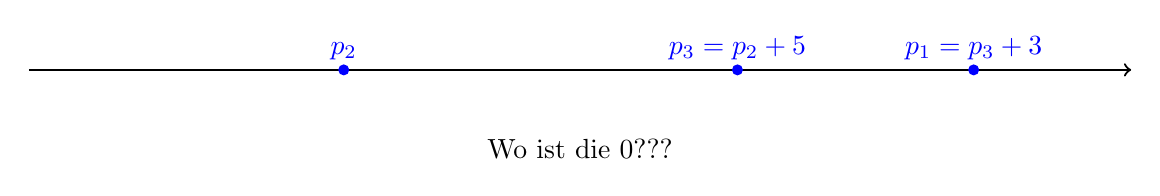
\begin{tikzpicture} 
	\draw[->,thick] (-7,0) -- (7,0);
	\fill[blue] (5,0) circle (0.07) node[above] {$p_1=p_3+3$};
	\fill[blue] (-3,0) circle (0.07) node[above]{$p_2$};
	\fill[blue] (2,0) circle (0.07) node[above]{$p_3=p_2+5$};
	\node at (0,-1) {Wo ist die $0$???};
\end{tikzpicture} 
\end{center} 

Trotz der Tatsache, dass die Positionen $(p_1,p_2,p_3)$ modulo $U$ keine exakten Angaben der Werte von $p_1, p_2, p_3$ sind, kann man modulo $U$ rechnen. Hat zum Beispiel nach einer Weile, das erste Auto $1$ Einheit, das zweite Auto $2$ Einheiten und das dritte Auto $4$ Einheiten zurückgelegt, so ergibt sich der Vektor der neuen Positionen $(5+1,-3+2,2+4) = (6,-1,6)$ modulo $U$: das dritte Auto hat das erste Auto eingeholt, das zweite liegt $7$ Einheiten zurück. Nach wie vor kennt man aber die durch die Angabe der Positionen modulo $U$ keine  Information über die genaue Positionen auf der Strecke. 
\end{bsp} 


\begin{bsp}[Ein weiterführendes Beispiel für Quotientenräume]
	Analog zu Polynomringen mit einer Unbestimmten kann man auch Polynomringe mit mehr als einer Unbestimmten einführen. Wir betrachten etwa $ \R[x,y] $ -- den Polynomring der Polynome in Unbestimmten $ x $ und $ y $ mit Koeffizienten in $ \R $:
	\begin{equation*}
		1, \quad 1 - 2xy + y^2, \quad xy + 3x^2 + x^4y^5 \quad \in \R[x,y]
	\end{equation*}
	$ \R[x,y] $ ist ein Vektorraum über $ \R $. (Rechnen auf dem Kreis:) $ U := \{ (x^2+y^2-1) \cdot f(x,y) : f(x,y) \in \R[x,y] \} $ ist ein Untervektorraum von $ \R[x,y] $. $ \R[x,y]/U $ entspricht einer Struktur in der mit Berücksichtigung der Bedingung $ x^2 + y^2 = 1 $ gerechnet wird.
	
	Etwa werden $ x + y $ und $ x + y + (x^2 + y^2 - 1) \cdot 2 $ gleich, wenn man $ x^2 + y^2 = 1 $ fordert. Genauer gilt:
	\begin{equation*}
		x + y \equiv x + y + (x^2 + y^2 -1) \cdot 2 \mod{U}
	\end{equation*}
\end{bsp}

\clearpage
\subsection{Koordinatensysteme}

\subsubsection{Basisdarstellung von Vektoren}

Sei $ V $ endlichdimensionaler Vektorraum über $ \K $ und sei $ n := \dim(V) $. Sei $ \mathcal{B} = (b_1, \ldots, b_n) $ eine Basis von $ V $ und $ x \in V $. Der Vektor $ (\beta_1, \ldots, \beta_n) \in \K^n $ mit $ x = \beta_1b_1 + \ldots + \beta_nb_n $ heißt der Vektor der Koordinaten von $ x $ in der Basis $ \mathcal{B} $. Bezeichnung: $ x_\mathcal{B} $.Die Abbildung $ x \mapsto x_\mathcal{B} $ von $ V $ nach $ \K^n $ ist eine lineare Bijektion.
\begin{bsp}[RoboCup Soccer]
Inhalt...
\end{bsp}

\subsubsection{Basiswechsel}

Sei $ V $ endlichdimensionaler Vektorraum über $ \K $ mit $ n := \dim(V) $. Seien $ \mathcal{A} = (a_1, \ldots, a_n) $ und $ \mathcal{B} = (b_1, \ldots, b_n) $ Basen von $ V $. Wir führen die Matrix 
\begin{equation}
T_{\mathcal{B} \ot \mathcal{A}} := \begin{pmatrix} 
| & & |
\\ (a_1)_{\mathcal{B}} & \cdots & (a_n)_{\mathcal{B}} 
\\ | & & | 
\end{pmatrix} 
\end{equation}
 ein, deren $ j $-te Spalte mit $ (a_j)_\mathcal{B} $ übereinstimmt ($ \forall j \in \is{1}{n} $). Das heißt, bei der Angabe durch die Komponenten
\begin{equation}
	T_{\mathcal{B} \ot \mathcal{A}} =
	\begin{pmatrix}
		\tau_{11} & \cdots & \tau_{1n} \\
		\vdots &   & \vdots \\
		\tau_{n1} & \cdots & \tau_{nn}
	\end{pmatrix}
\end{equation}
erfüllen die Komponenten die Gleichungen
\begin{equation}
	a_j = \tau_{1j}b_1 + \ldots + \tau_{nj}b_n \quad \forall i \in \is{1}{n}.
\end{equation}
für $j \in \{1,\ldots,n\}$. 

Die Matrix $ T_{\mathcal{B} \ot \mathcal{A}} $ heißt \emph{Basiswechselmatrix} oder \emph{Matrix des Wechsels} von der Basis $ \mathcal{A} $ zur Basis $ \mathcal{B} $. Hier ist $\mathcal{A}$ die ``alte Basis''und $\mathcal{B}$ die ``neue Basis''. Durch die Matrix $ T_{\mathcal{B} \ot \mathcal{A}} $ werden also die Vektoren der alten Basis in der neuen Basis geschrieben. Diese Beschreibungen helfen beim Übergang von der alten zur neuen Basis: 

\begin{thm}
	Sei $ V $ endlichdimensionaler Vektorraum über $ \K $, seien $ \mathcal{A} $ und $ \mathcal{B} $ Basen von $ V $ und sei $ x \in V $. Dann gilt:
	\begin{equation}
		x_\mathcal{B} = T_{\mathcal{B} \ot \mathcal{A}} x_\mathcal{A}.
	\end{equation}
\end{thm}
\begin{proof}
	Seien $ \begin{aligned}[t] x_\mathcal{A} = (\alpha_1, \ldots, \alpha_n), x_\mathcal{B} = (\beta_1 \ldots, \beta_n), T_{\mathcal{B} \ot \mathcal{A}} = (\tau_{ij})_{i,j=1}^n \end{aligned} $. D.h.
	\begin{align*}
		x &= \alpha_1a_1 + \ldots + \alpha_na_n \\
		&= \beta_1b_1 + \ldots + \beta_nb_n \\
		a_j &= \tau_{1j}b_1 + \ldots + \tau_{nj}b_n \quad \forall j.
	\end{align*}
	Es folgt:
	\begin{align*}
		x &= \sum\limits_{j=1}^n \alpha_ja_j \\
		&= \sum\limits_{j=1}^{n} \alpha_j \left( \sum\limits_{i=1}^{n} \tau_{ij}b_i \right) \\
		&= \sum\limits_{i,j \in \is{1}{n}} \tau_{ij}\alpha_jb_i \\
		&= \sum\limits_{i=1}^{n} \left( \sum\limits_{j=1}^{n} \tau_{ij}\alpha_j \right) b_i.
	\end{align*}
	Andererseits gilt $ x = \sum_{i=1}^n \beta_ib_i $. Es folgt $ \beta_i = \sum_{j=1}^n \tau_{ij}\alpha_j $ für alle $ i \in \is{1}{n} $. Mit anderen Worten gilt $ x_\mathcal{B} = T_{\mathcal{B} \ot \mathcal{A}} x_\mathcal{A} $.
\end{proof}

\subsubsection{Wiederholter Basiswechsel}

\begin{thm}
	Sei $ V $ endlichdimensionaler Vektorraum über $ \K $ und seien $ \mathcal{A}, \mathcal{B} $ und $ \mathcal{C} $ Basen von $ V $. Dann gilt:
	\begin{equation}
		T_{C \ot A} = T_{C \ot B} T_{b \ot A}.
	\end{equation}
\end{thm}
\begin{proof}
	Übung.
\end{proof}

\begin{klr}
	Sei $ V $ endlichdimensionaler Vektorraum über $ \K $ und seien $ \mathcal{A} $ und $ \mathcal{B} $ Basen von $ V $. Dann ist $ T_{B \ot A} $ invertierbar und es gilt:
	\begin{equation}
		\left( T_{B \ot A} \right)^{-1} = T_{A \ot B}.
	\end{equation}
\end{klr}
\begin{proof}
	$ T_{A \ot A} $ ist die Einheitsmatrix. Die Behauptung folgt aus dem vorigen Theorem mit $ \mathcal{C} = \mathcal{A} $.
\end{proof}

\subsubsection{Basendarstellung von linearen Abbildungen}

Seien $ V $ und $ W $ endlichdimensionale Vektorräume über $ \K $. Sei $ m := \dim(W) $ und $ n := \dim(V) $. Sei $ \mathcal{A} = (a_1, \ldots, a_m) $ Basis von $ W $ und $ \mathcal{B} = (b_1, \ldots, b_n) $ Basis von $ V $. Sei $ F : V \to W $ linear.

Wir definieren die Matrix $ F_\mathcal{A,B} = (\phi_{ij}){}_{i=1}^m{}_{j=1}^n \in \K^{m \times n} $, deren $ j $-te Spalte mit $ F(b_j)_\mathcal{A} $ übereinstimmt (für alle $ j \in \is{1}{n} $). D.h.
\begin{equation}
	F_\mathcal{A,B} =
	\begin{pmatrix}
		\phi_{11} & \cdots & \phi_{1n} \\
		 &  \vdots &  \\
		\phi_{m1} & \cdots & \phi_{mn}
	\end{pmatrix}
\end{equation}
und
\begin{equation}
	F(b_j) = \phi_{1j}a_1 + \ldots + \phi_{mj}a_m \quad \forall j \in \is{1}{n}.
\end{equation}

\begin{thm}
	Seien $ V $ und $ W $ endlichdimensionale Vektorräume über $ \K $, sei $ \mathcal{A} $ Basis von $ W $ und $ \mathcal{B} $ Basis von $ V $. Sei $ F : V \to W $ linear. Sei $ x \in V $ und $ y = F(x) $. Dann gilt:
	\begin{equation}
		y_\mathcal{A} = F_\mathcal{A,B} x_\mathcal{B}.
	\end{equation}
\end{thm}
\begin{proof}
	Sei $ \mathcal{B} = (b_1, \ldots, b_n) $. Sei $ \mathcal{A} = (a_1, \ldots, a_m) $. Sei $ F_{\mathcal{A},\mathcal{B}} = (\phi_{ij}){}_{i=1}^m{}_{j=1}^n $. Sei $ x_\mathcal{B} = (\beta_1, \ldots, \beta_n) $, d.h. $ x = \beta_1b_1 + \ldots + \beta_nb_n $. Sei $ y_\mathcal{A} = (\alpha_1, \ldots, \alpha_n) $, d.h. $ y = \alpha_1a_1 + \ldots + \alpha_na_n $.
	\begin{align*}
		y &= F(x) = F(\beta_1b_1 + \ldots + \beta_nb_n) = \beta_1F(b_1) + \ldots + \beta_nF(b_n) \\
		&= \sum\limits_{j=1}^{n} \beta_j F(b_j) = \sum\limits_{j=1}^{n} \beta_j \left( \sum\limits_{i=1}^{m} \phi_{ij}a_i \right) = \sum\limits_{i=1}^{m} \left( \sum\limits_{j=1}^{n} \phi_{ij}\beta_j \right) a_i.
	\end{align*}
	Andererseits gilt $ y = \sum_{i=1}^m \alpha_ia_i $. Es folgt $ \alpha_i = \sum_{j=1}^{n} \phi_{ij}\beta_j $ für alle $ i \in \is{1}{m} $. D.h. $ y_\mathcal{A} = F_\mathcal{A,B} x_\mathcal{B} $.
\end{proof}

$ F_{\mathcal{A},\mathcal{B}} $ heißt die Darstellung von $ F $ in $ \mathcal{A} $ und $ \mathcal{B} $. Die Abbildung $ F \mapsto F_{\mathcal{A},\mathcal{B}} $ ist eine lineare Bijektion von $ \Lin(V,W) $ nach $ \K^{m \times n} $.

Für lineare Abbildungen $ F : V \to V $ und Basen $ \mathcal{B} $ von $ V $ führen wir die Bezeichnung $ F_\mathcal{B} := F_\mathcal{B,B} $ ein.

\subsubsection{Basendarstellung einer Komposition von linearen Abbildungen}

\begin{thm}
	Seien $ U, V $ und $ W $ endlichdimensionale Vektorräume über $ \K $. Seien $ F : V \to W $ und $ G : U \to V $ linear. Sei $ \mathcal{A} $ Basis von $ W $, $ \mathcal{B} $ Basis von $ V $ und $ \mathcal{C} $ Basis von $ U $. Dann gilt:
	\begin{equation}
		(F \circ G)_\mathcal{A,C} = F_\mathcal{A,B} \cdot F_\mathcal{B,C}.
	\end{equation}
\end{thm}
\begin{proof}
	Übung (?), folgt aus dem vorigen Theorem.
\end{proof}

\subsubsection{Basiswechsel für lineare Abbildungen}

\begin{thm}
	Seien $ V $ und $ W $ endlichdimensionale Vektorräume über $ \K $. Seien $ \mathcal{A} $ und $ \mathcal{A'} $ Basen von $ W $. Seien $ \mathcal{B} $ und $ \mathcal{B'} $ Basen von $ V $. Sei $ F : V \to W $ linear. Dann gilt:
	\begin{equation}
		F_\mathcal{A',B'} = T_{\mathcal{A'} \ot \mathcal{A}} \cdot F_\mathcal{A,B} \cdot T_{\mathcal{B} \ot \mathcal{B'}}
	\end{equation}
\end{thm}
\begin{proof} 
	Sei $ x \in V $ und $ y = F(x) $. Es gilt $ y_\mathcal{A} = F_\mathcal{A,B} \cdot x_\mathcal{B} $ und $ y_\mathcal{A'} = F_\mathcal{A',B'} \cdot x_\mathcal{B'} $. Mit der Verwendung von $ x_\mathcal{B} = T_{\mathcal{B} \ot \mathcal{B'}} \cdot x_\mathcal{B'} $ folgt $ y_\mathcal{A} = F_\mathcal{A,B} \cdot T_{\mathcal{B} \ot \mathcal{B'}} \cdot x_\mathcal{B'} $. Multiplikation mit $ T_{\mathcal{A'} \ot \mathcal{A}} $ von links ergibt $ y_\mathcal{A'} =  T_{\mathcal{A'} \ot \mathcal{A}} \cdot y_\mathcal{A} = T_{\mathcal{A'} \ot \mathcal{A}} \cdot F_\mathcal{A,B} \cdot T_{\mathcal{B} \ot \mathcal{B'}} \cdot x_\mathcal{B'} $. Es folgt $ F_\mathcal{A',B'} \cdot x_\mathcal{B'} = T_{\mathcal{A'} \ot \mathcal{A}} \cdot F_\mathcal{A,B} \cdot T_{\mathcal{B} \ot \mathcal{B'}} \cdot x_\mathcal{B'} $. Sei $ \mathcal{B'} = (b'_1, \ldots, b'_n) $. Im Fall $ x = b'_i $ gilt $ x_\mathcal{B'} = e_i $. Die vorige Gleichung ergibt, dass die $ i $-ten Spalten von $ F_\mathcal{A',B'} $ und $ T_{\mathcal{A'} \ot \mathcal{A}} \cdot F_\mathcal{A,B} \cdot T_{\mathcal{B} \ot \mathcal{B'}} $ übereinstimmen. Weil $ i $ beliebig ist, folgt die Behauptung.
\end{proof}
